\section{Background}

Most of the literature on the topic addresses coevolution in one of two ways, depending on the initial assumptions. One may begin without the assumption coevolution has occurred, and then ascertain the likelihood that it did. Or, having established that coevolution has occurred either by testing for it or through some other piece of exogenous evidence, one may ascertain what history is most likely. The first approach frames the question as, {\em How likely is it that these two interacting groups have coevolved?} The second frames the question as, {\em Given that these two interacting groups have coevolved, what is the most likely sequence of events?} The first approach yields an overall likelihood, and the second yields a sequence of events (host switches, extinctions and bifurcations) that may have resulted in the observed associations. These two approaches are covered in sections \ref{FP_phylosig} and \ref{FP_permutation}, respectively.

We are interested in learning about the natural history of the system, and so we would like to ask a somewhat enlarged question. {\em In a system where the hosts are associated with a very large number of related organisms, which clades show evidence of coevolution with the hosts?} We will focus on this approach, which is summarized in section \ref{FP_spectral_summary}. 

For each organism that appears among the microbiomes of a group of hosts, there exists a pattern of observed associations between the ``guest'' organisms and the host organisms. These associations can be treated as traits of the host, and the history of each association can be examined like any phenotypic trait of the host. Alternatively, the tendency to associate (or not) with a host could be treated as a trait distributed over a group of microbial organisms, although it would require dividing the microbiome into groups of related OTUs in order to be meaningful. Association with a particular host is more likely to correspond to different traits for more distantly related OTUs, and so it is probably not meaningful to naively apply stochastic trait mapping across all bacterial diversity.

%In {\em Analysis of phylogenetics and evolution with {\tt R}} (p. 236), Emmanuael Paradis describes phylogenetic signal as follows :

%\begin{quote}
%The concept of phylogenetic signal is at the heart of most phylogenetic methods. From a statistical point of view, a phylogenetic signal is defined by the non-null covariances (i.e., non-independence) among species. From a biological point of view, phylogenetic signal is a direct consequence of the evolution of traits and its form will depend on the evolutionary mechanisms in action.
%\end{quote}

\subsection{Tests for phylogenetic signal}\label{FP_phylosig}

By treating OTUs, or groups of OTUs, as traits of the hosts, one can apply a variety of methods for estimating how likely it is that a trait is both conserved and vertically transmitted. These measures of ``phylogenetic signal,'' attempt to characterize the statistical independence (or autocorrelation) among species traits due to phylogenetic relatedness. The less the trait distribution can be said to be statistically independent from the phylogeny, the more phylogenetic signal is present in that trait. \cite{felsenstein1985phylogenies} M{\"u}nkem{\"u}ller {\em et al.} \cite{munkemuller2012measure} have prepared an excellent review covering the theory and application of Abouheif's $C_{mean}$, Pagel's $\lambda$, Moran's $I$, Blomberg's $K$ and some of their variations. Unfortunately, trait-based models do not account for interactions {\em among} traits, or a way to account for traits that have their own evolutionary model (i.e., traits that are themselves organisms). For an interaction of a particular host and microbe, this might not present a problem. For examining interactions of microbiomes (or a significant subset of one), the assumption that traits are distributed independently is a significant weakness. 

\subfile{FishPoo/figures/figure4}

Individual OTUs may represent several distinct organisms, each with their own pattern of association. Figure \ref{fig:FP_fig4}) illustrates an example from the Cichlids dataset where this is likely the case. The taxonomic assignments suggest that the second OTU ({\tt CHALBRI1\_4931}) may represent a more diverse group of organisms than the first ({\tt CHALBRI1\_1198}). If more than one organism belonging to Enterobacteriaceae is present, then it is likely that each would have a different pattern of relationships with the host organisms. The sum of these patterns is likely to have a lower phylogenetic signal than any particular one of them, and could account for the lower phylogenetic signal observed for this OTU. In principle, one could compensate for the different levels of diversity represented by different 16S sequences, but any such approach would require a relatively complete and unbiased database of microbial diversity. Unfortunately, such a database does not yet exist.

\subsection{Permutation tests for cospeciation}\label{FP_permutation}

Where phylogeneitic signal estimates the non-independence of a trait from the phylogeny of the organisms among which it is distributed, other methods exist for estimating the non-independence of interacting phylogneies from one another. For example, Hafner {\em et al.} \cite{hafner1994disparate} examine the relationship between pocket gophers and their chewing louse parasites using a tree reconciliation test implemented in {\tt COMPONENT} by Roderic D. M. Page \cite{page1993genes}. This is, in essence, a parsimony approach; the gene duplication and loss events necessary to achieve topological congruence between two trees are minimized. Hafner {\em et al.} first reject the null hypothesis (independent evolution) by applying the tree reconciliation test among gopher, louse and randomly drawn trees, and then examine rates of nucleotide divergence between the gopher and louse. This dataset has since been reanalyzed in many other publications, has become a sort of base-case for co-diversification methods. Notably, Huelsenbeck {\em et al.} use the gopher/louse data set to introduce the use of Bayesian inference to cospeciation. \cite{huelsenbeck2000bayesian} In the context of a microbiome where many nested interactions must be examined, parsimony methods are inapplicable due to a lack of statistical consistency, \cite{felsenstein1978cases} and Bayesian methods due to their large computational demands.

Hommola {\em et al.} \cite{hommola2009permutation} describe a method to extend the Mantel test. \cite{mantel1967detection} The Mantel test is a statistic on the correlation of two matrixes, and requires that the matrixes be of equal rank. When applied to distance matrixes for trees containing differing numbers of taxa, one must delete or duplicate taxa until the matrix ranks are equal. This results in anomalous results which Hommola {\em et al.} explore in detail. To address this issue, they take every pair of linked tips (e.g., a parasite species that is observed to associate with a host species), and examine the correlation of distances through the two trees. This accommodates trees of arbitrary size and arbitrary patterns of association among their tips, and can be coupled with a straightforward permutation test to estimate the significance of the correlations. One can walk through every clade in the phylogeny of host-associated OTUs and, for every clade, compute the Hommola correlation with the host phylogeny (Figure \ref{FP_hommola_corr}). 

\subfile{FishPoo/figures/figure5}

However, there are some important difficulties when it comes to applying the Hommola cospeciation test to a large number of clades belonging to the same tree. First of all, this approach necessarily entails multiple comparisons, and so a correction to the significance values is required. However, a Bonferroni correction is not appropriate because the structure of each clade is not independent of the others. Rather, they are hierarchically nested within a tree, itself inferred from an probabilistic model (an approximate maximum likelihood model, in this case) based on nucleotide transitions inferred from an alignment. The autocorrelation within the tree would need to be accounted for, but calculating it would not be straightforward. At a minimum, one would need to take into account the fact that the multiple comparisons have hierarchical relationships.

The second difficulty arises from the need to perform unsupervised correlation tests. Hommola {\em et al.} use the Pearson product-moment correlation, which assumes that the processes are independent, identically distributed, and follow a bivariate normal distribution. Unfortunately, there is reason to suppose that the distances among tips of a phylogenetic tree would be normally distributed. Of course, other correlation statistics could be substituted at the expense of computational complexity (Spearman's rank correlation coefficient, for example, obeys quadratic scaling), but the number of OTUs present in a typical microbiome would call for the use of a supercomputer.

\subfile{FishPoo/figures/figure6}

The reliance on a summary statistic in Hommola {\em et al} makes detecting co-diversification in the microbiome difficlt. All summary statistics are a form of information reduction, usually a projection into a 1-dimensional space, and their interpretation depends on structural properties within the data. While it is often possible to construct complimentary tests to insure that assumptions hold, those tests are themselves likely to rely on summary statistics. Ultimately, someone has to actually inspect the data to make sure that the correlations are meaningful. \cite{anscombe1973graphs} For example, compare the distribution of pairwise distances for the Gopher/Louse dataset \cite{hafner1994disparate} to Clade 72223, which appears just below it in Figure \ref{FP_highcorr}. Both have about the same correlation coefficient ($r=0.490$ verses $r=0.488$), very high significance ($1.38\times 10^{-9}$ verses $p=3.21\times 10^{-223}$ and are within an order of magnitude in size ($15 \times 17$ verses $14 \times 68$). Nevertheless, the two distributions are obviously different, and the vertical banding pattern in Clade 72223 is strongly reminiscent of Case 4 in Anscombe's quartet. The structural differences between these interactions can also be seen clearly when represented as tanglegrams (Figure \ref{fig:FP_tangles}).

\subfile{FishPoo/figures/figure7}

In principle, one could develop a hierarchical Bonferroni correction, design correlation tests that exclude artifactual features that crop up in distributions of patristic distances, and obtain the use of a powerful supercomputer. However, a third difficulty remains. All of the approaches mentioned so far are based upon an idealized model of coevolution. In the ideal case, the host and the guest organisms would diverge in lockstep and exhibit phylogenies of perfectly congruent structure. One might imagine this to be the case for vertically transmitted symbionts, but the reality is that it is not even true for different genes within the same organism (for example, due to incomplete lineage sorting). Coevolution can be expected to manifest alongside other effects. For example, a Red Queen interaction may ``leak'' lineages that escape from the reciprocal selective effects. A Red Queen interaction may emerge from a non-coevolutionary interaction, producing a embedded coevolution event. Organisms outside a coevolutionary interaction may impinge on the process, as may abiotic factors.

The model, and the statistical tests applied to it, must be sensitive enough to detect coevolution from a background of other process and selective enough to discriminate real cases of coevolution from patterns exhibiting spurious or artifactual resemblance to coevolution.

As mentioned before, the Gopher/Louse dataset from Hafner {\em et. al.} exhibits a Hommola correlation of $r=0.49$, which is rather poor as correlated processes go. Nevertheless, the ecological case for cospeciation is solid and its physiological basis is sound. The Sedge/Smut interaction from Escudero \cite{escudero2015phylogenetic} is also well established, but has a Hommola correlation of only $r=0.15$. By itself, the Hommola test is neither sensitive nor selective enough to identify coevolution in microbiomes. However, it does measure an informative structural property of interacting phylogenies. Viewed in a broader context, it is a valuable feature to include in a more generalized framework for classifying these interactions.

\subsection{Laplacian spectral density as a metric on phylogenetic topology}\label{FP_spectral_summary}

All four tests for phylogenetic signal are metrics for estimating the autocorrelation of a trait distribution with respect to the topology of a phylogenetic tree. The Hommola correlation test is a metric for estimating the autocorrelation of two trees. All five methods essentially sample the statistical {\em effect} of tree topology. There are mathematical approaches for interrogating the topology of trees, and graphs in general, that can make use of a greater portion of information present. One approach is examine moments of the spectral density distribution the graph Laplacian. The graph Laplacian is constructed by subtracting the graph adjacency matrix (Fig. \ref{FP_adjacency}) from the degree matrix (the total connectivity of each node). This representation of a general graph is often useful in graph analysis. For example, it can be used to calculate the number of spanning trees for the graph using Kirchhoff's theorem, and its second second smallest eigenvalue can be used to approximate to the sparsest cut through a given graph via Cheeger's inequality. 

\begin{figure}
\centering
\begin{subfigure}[t]{0.40\textwidth}
\begin{minipage}{0.40\textwidth}
\begin{tikzpicture}[every tree node/.style={draw,circle},
   level distance=2.8cm,sibling distance=0.7cm,
   edge from parent path={(\tikzparentnode) -- (\tikzchildnode)}]
\Tree
[.a
    \edge node[auto=right] {$\alpha$};
    [.b 
       \edge node[midway,left] {$\beta$};
       [.d ]
       \edge node[midway,right] {$\gamma$};
       [.e ]
        ]
    \edge node[auto=left] {$\delta$};
    [.c 
        \edge node[midway,left] {$\epsilon$};
        [.f ]
        \edge node[midway,right] {$\zeta$};
        [.g ]
        ]
]
\end{tikzpicture}
\end{minipage}
\end{subfigure}
\begin{subfigure}[t]{0.40\textwidth}
\begin{minipage}{0.40\textwidth}
\begin{equation*}
A =
\bordermatrix{
           & \mathrm{a} & \mathrm{b} & \mathrm{c} & \mathrm{d} & \mathrm{e} & \mathrm{f} & \mathrm{g} \cr
\mathrm{a} & 0          & \alpha     & \delta     & 0          & 0          & 0          & 0          \cr
\mathrm{b} & \alpha     & 0          & 0          & \beta      & \gamma     & 0          & 0          \cr
\mathrm{c} & \delta     & 0          & 0          & 0          & 0          & \epsilon   & \zeta      \cr
\mathrm{d} & 0          & \beta      & 0          & 0          & 0          & 0          & 0          \cr
\mathrm{e} & 0          & \gamma     & 0          & 0          & 0          & 0          & 0          \cr
\mathrm{f} & 0          & 0          & \epsilon   & 0          & 0          & 0          & 0          \cr
\mathrm{g} & 0          & 0          & \zeta      & 0          & 0          & 0          & 0          \cr
}
\end{equation*}
\end{minipage}
\end{subfigure}
\caption{Construction of the graph adjacency matrix for a phylogenetic tree.}
\label{FP_adjacency}
\end{figure}

The eigenvalues of the graph Laplacian, sometimes called the Laplacian spectrum, correspond to the frequency with which a random walker would visit each node in steady state (i.e., in the limit of the number of random steps as the number of steps approaches infinity). It is important to note that the Laplacian spectrum of a graph is not unique. Graphs that have the same spectrum but are not isomorphic (i.e., do not have the same structure) are said to be isospectral or cospectral. For trees of intermediate size ($ \approx 5 < n < n \rightarrow \infty$), the probability that two randomly selected trees will share the same spectrum is finite but negligible. \cite{matsen2012ubiquity} Most phylogenetic trees that express useful information fall within this range, and so the Laplacian spectrum can serve as a good description of a trees's general and local topology.

To compare the topology of two trees that have different numbers of nodes, it is necessary to do something about the fact that they will have different numbers of eigenvalues. Matsen and Evans \cite{matsen2012ubiquity} solve this problem by projecting the eigenvalues into a continuous 1-dimensional space using a kernel density estimator (KDE). The distributions produced by the KDE can then be compared directly. Lewitus and Morlon \cite{lewitus2015characterizing} use the Shannon-Jensen divergence between distributions, as well as several moments of the distributions, to estimate the topological dissimilarity among trees.  

This suggests a spectral approach to coevolution problems. It is relatively straightforward to obtain the Shannon-Jensen divergence between a the phylogeny of a group of hosts and their parasites. However, interpretation of the result is not so straightforward. How much divergence is required to disqualify a pair of trees from being ``similar'' in topology? How sensitive is the divergence to tree size? How does one establish confidence intervals on this metric? Moreover, the divergence between the two trees does not take into account the way that the organisms in the trees interact with one another. 

To address these questions, we propose four extensions to this approach. First, it is necessary to construct a generalized graph representing {\em both} trees. Second, the ecological interactions between the organisms represented in the trees are incorporated into the graph. Third, the phylogenetic distances in the trees are normalized with respect to one another and with respect to other interactions; we do this by setting the total distance in each tree from root to deepest tip to unity, and the links between the trees to the average of all branch lengths in each tree. Fourth, instead of looking for endogenous evidence of coevolution within an interaction, we compare interactions with unknown ecology to those with known ecology. By using a comparative approach, contextual information that would be difficult to obtain (and would likely result in overfitting) in a model-based approach can be integrated and tested as a supervised machine learning problem.

It is worth noting that almost all trees are cospectral, \cite{schwenk1973almost} whereas only a subset of generalized graphs are cospectral (uniform star graphs and complete graphs, for example). Spectral classification of graphs should thus suffer a lower rate of collisions in spectral space than trees alone. 